Il s'agit du scénario A dans lequel, à la fin de l'achat de l'énergie, le client demande à faire vérifier le numéro de suivi de l'énergie achetée. Cela signifie qu'il faut valider le CRACHA et le CRADO qu'il contient auprès de l'AMI qui est l'autorité de certification.
\\[1cm]
 Ce scénario n'a pas été traité dans notre projet, mais voici à quoi cela aurait du ressemblé :
\\
 \begin{figure}[h]
    \centering
    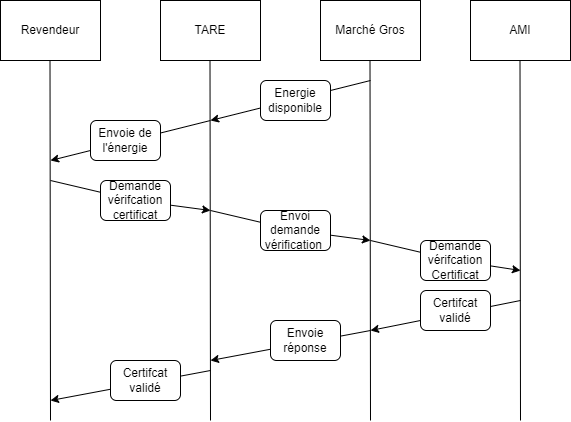
\includegraphics[width=130mm, height=100mm]{images/ScenarioA2.png}
    \caption{Schéma du scénario A2}
    \label{img:mesh22}
\end{figure}
\newpage